% 输出PDF时,需要把所有路径.替换成.
\documentclass{beamer}
\usepackage[UTF8,noindent]{ctex}
\usetheme{Berkeley}
\usecolortheme{seagull}

% 导言
\title{组会汇报}
\subtitle{移动机器人远程交互软件设计与实现}
\institute{C400}
\author{黎振胜}
\date{\today}
\subject{中南大学研究生学位论文}
\keywords{移动机器人,人机交互,UML,LabVIEW,ROS}

\logo{
\includegraphics[width=1.54cm]{./resource/logo/csu.pdf}}

\begin{document}

\begin{frame}
\maketitle
\end{frame}
%--- Next Frame ---%
\begin{frame}[t]{汇报内容}
    \tableofcontents
\end{frame}
%--- Next Frame ---%
\begin{frame}[t]{1.1背景}
    \section{背景和总体方案}
    \subsection{背景}
    \begin{itemize}
        \item 移动机器人代替人去危险场合执行探测和救援任务的应用背景
            \begin{itemize}
                \item 远场控制;数据可视化;指令传输
                \item 机器人具有一定自主性
            \end{itemize}
        \item 为机器人提供人机交互界面
            \begin{itemize}
                \item LabVIEW软件的优势,具有大量的内置控件
            \end{itemize}
        \item 设备,算法的快速集成
            \begin{itemize}
                \item 部署自然语言交互,决策,规划等算法
                \item 快速连接手柄等设备
            \end{itemize}
    \end{itemize}
\end{frame}
%--- Next Frame ---%
\begin{frame}[t]{1.2总体方案}
    % \subsection{总体方案}
    \only<1>{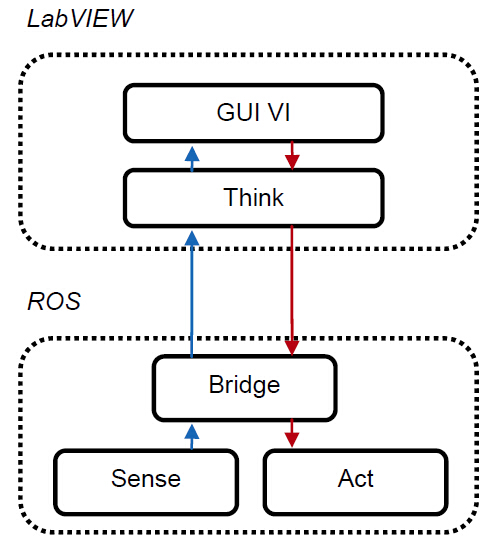
\includegraphics[scale=0.5]{./resource/graph/LabVIEW-control-ros-enabled-robot.jpg}}
    \only<2>{硬件表示}
    \only<2>{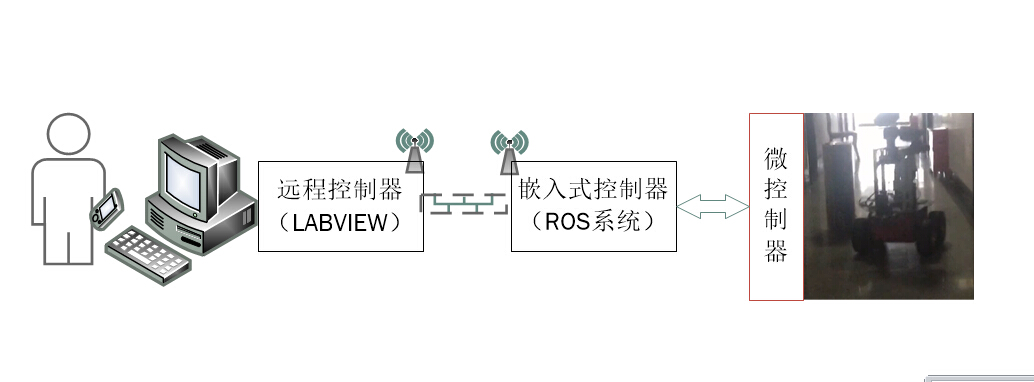
\includegraphics[scale=0.40]{./resource/graph/2-visio2010.jpg}}
    \only<3>{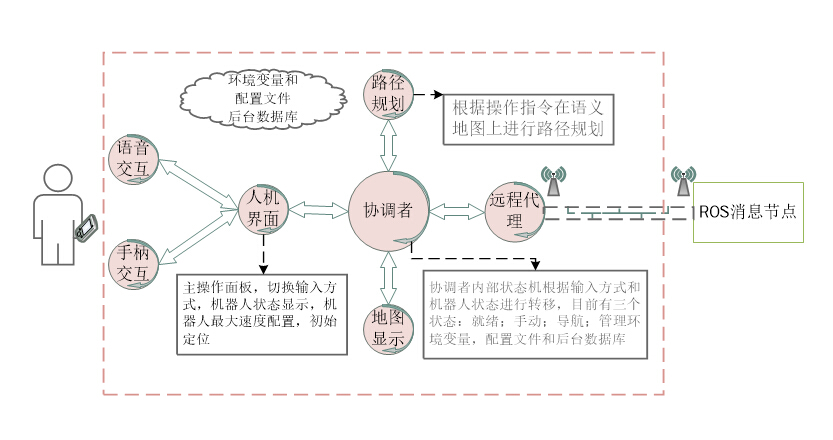
\includegraphics[scale=0.5]{./resource/graph/3-visio2010.jpg}}
\end{frame}
%--- Next Frame ---%
\begin{frame}[t]{方案特点}
    \subsection{特点}
    \begin{enumerate}
        \item 提供三种人与机器人交互的接口并可在三种方式下自由切换
        \item 自然语言交互接口,手柄遥操作接口和地图导引接口
        \item 提供与基于ROS的远程机器人自律控制的命令交互及传感信息接口
        \item 提供其它的智能计算模块接口,如用于上层逻辑推演的计算模块、用于视觉图像识别的计算模块等
        \item 提供机器人位置的实时地图显示功能
        \item 基于组件的软件系统设计和基于操作者框架的LabVIEW程序实现
    \end{enumerate}
\end{frame}
%--- Next Frame ---%
\begin{frame}[t]{2.1使用LabVIEW Actor Framework进行程序设计}
    \section{基于LabVIEW的远程交互平台软件设计和实现}
    \subsection{LVAF}
    \begin{itemize}
        \item 是什么
            \begin{itemize}
                \item 是一种基于消息机制的进程间通信框架
            \end{itemize}
        \item 为什么
            \begin{itemize}
                \item 模块化和扩展性
                \item 并发效率高
            \end{itemize}
        \item 理解LVAF
            \begin{itemize}
                \item 打开LabVIEW官方样例程序
            \end{itemize}
    \end{itemize}
\end{frame}
%--- Next Frame ---%
\begin{frame}[t]{一个例子理解LVAF}
    \begin{itemize}
        \item 并发
        \item 进程间通信
        \item 消息和事件
    \end{itemize}
    \begin{center}
        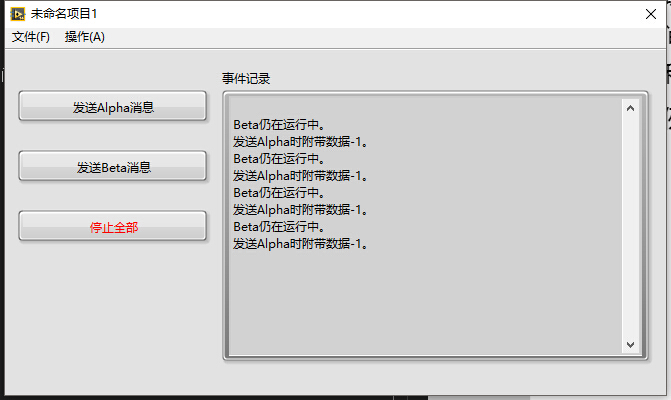
\includegraphics[scale=0.5]{./resource/graph/actor-framework.jpg}    
    \end{center}
\end{frame}
%--- Next Frame ---%
\begin{frame}[t]{例子程序的LVAF组成}
    \only<1>{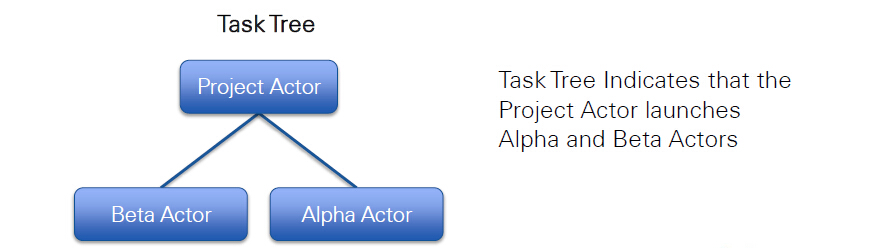
\includegraphics[scale=0.5]{./resource/graph/example-tasktree.jpg}}
    \only<2>{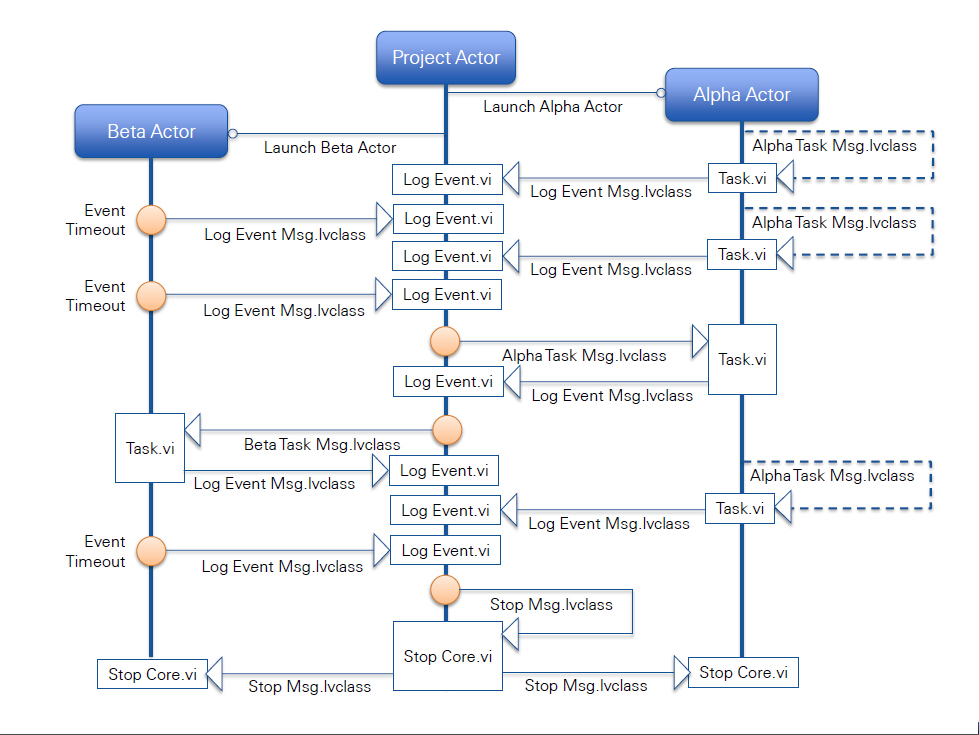
\includegraphics[scale=0.4]{./resource/graph/example-communication.jpg}}
\end{frame}
%--- Next Frame ---%
\begin{frame}[t]{本软件平台的LVAF组成}
    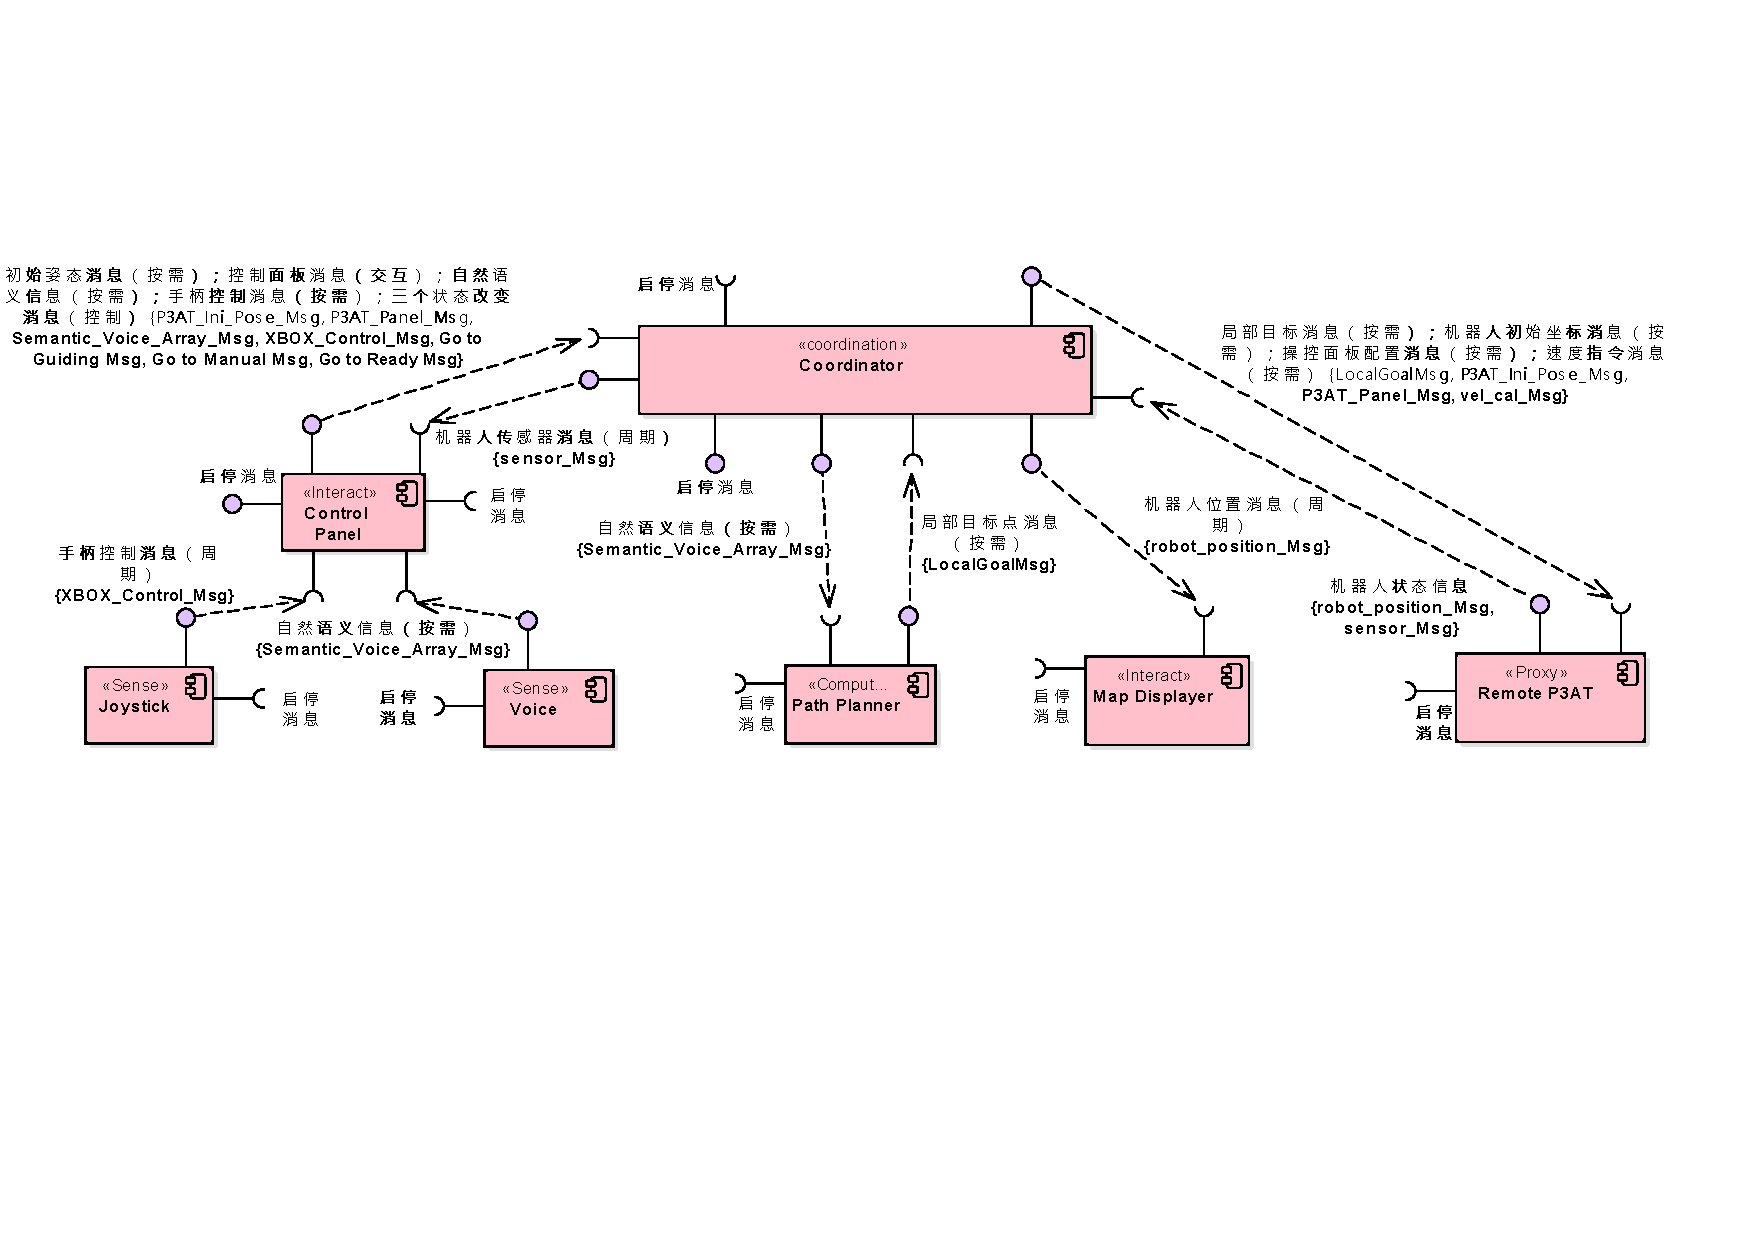
\includegraphics[scale=0.38]{./resource/graph/5.pdf}
    有哪些消息,消息如何传递
\end{frame}
%--- Next Frame ---%
\begin{frame}[t]{状态设计模式:State Actor}
    \only<1>{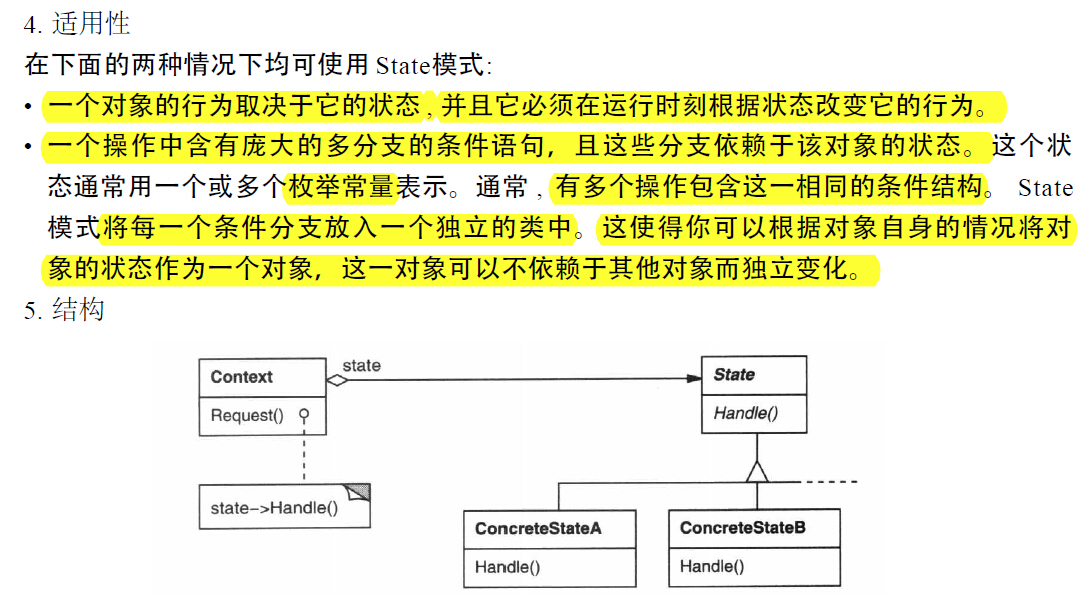
\includegraphics[scale=0.36]{./resource/graph/state-pattern.jpg}}
    \only<1>{   多状态,每一个状态下完成不同的任务}
    \only<2>{多状态,每一个状态下对不同的消息有不同的响应}
    \only<2>{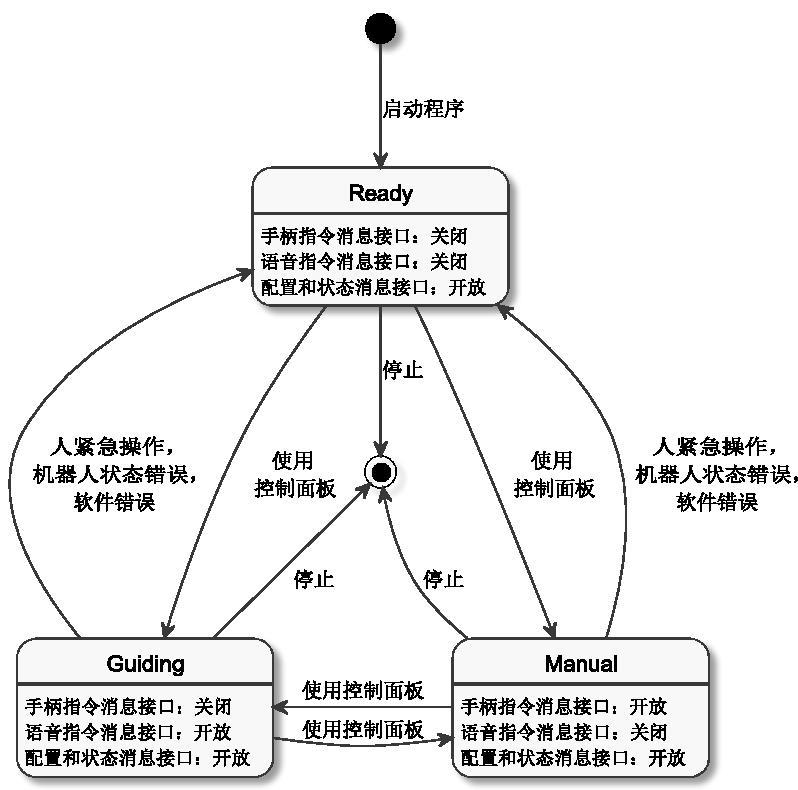
\includegraphics[scale=0.5]{./resource/graph/7.pdf}}
\end{frame}
%--- Next Frame ---%
\begin{frame}[t]{软件界面}
    \only<1>{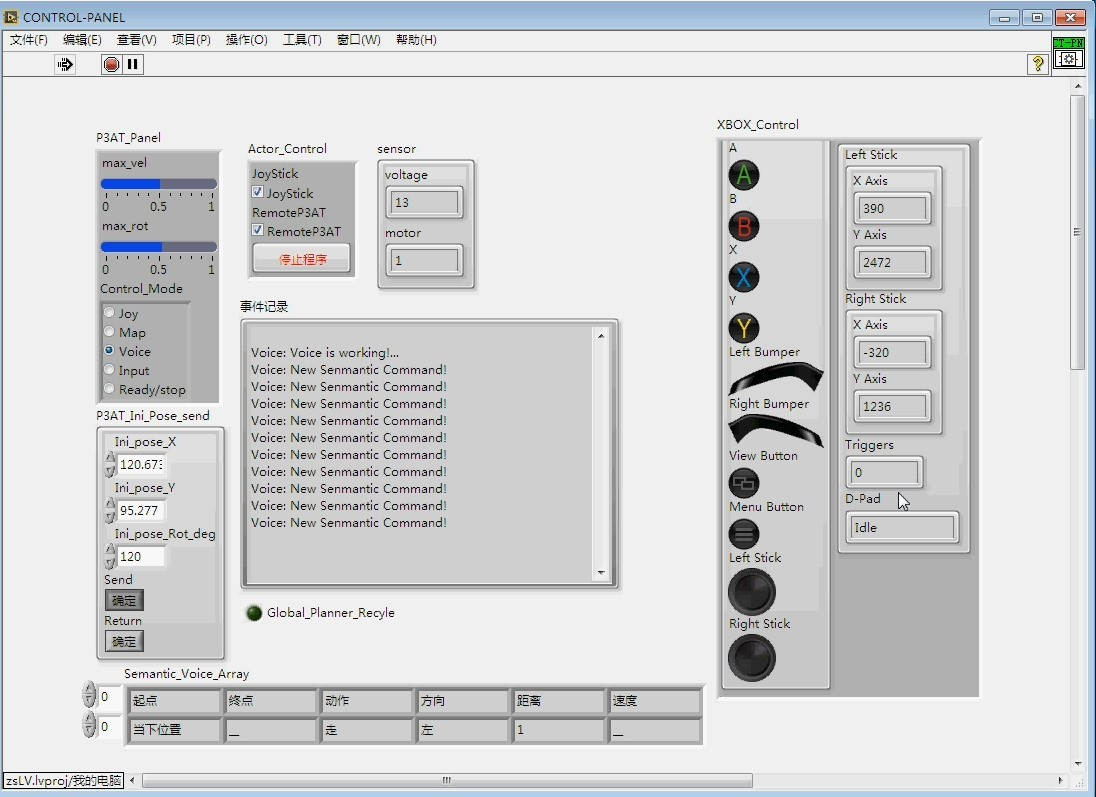
\includegraphics[scale=0.35]{./resource/graph/11.jpg}}
    \only<2>{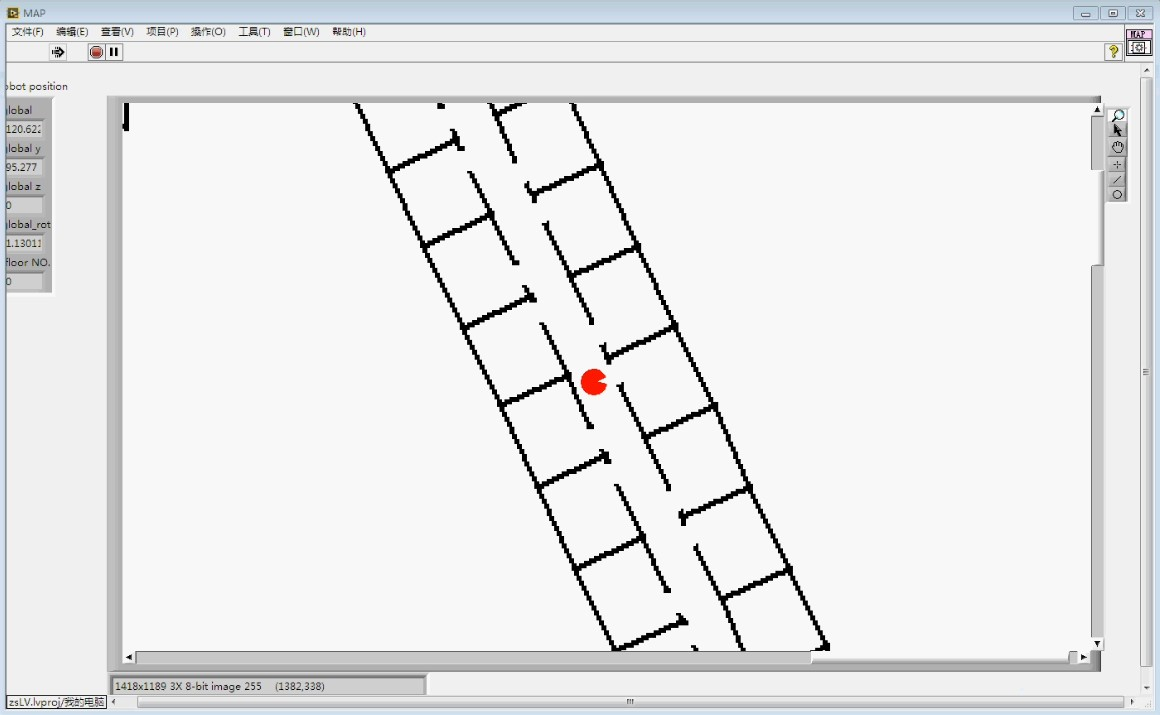
\includegraphics[scale=0.35]{./resource/graph/12.jpg}}
\end{frame}
%--- Next Frame ---%
\begin{frame}[t]{2.2远程人机交互软件设计的UML描述}
    \subsection{UML}
    \begin{itemize}
        \item Universal Modeling Language:面向对象程序的通用建模语言
        \item 为什么要用UML
            \begin{itemize}
                \item 描述
                \item 交流
                \item 策划
            \end{itemize}
    \end{itemize}
    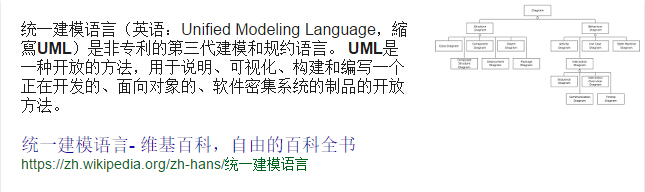
\includegraphics[scale=0.6]{./resource/graph/UML-google.jpg}
\end{frame}
%--- Next Frame ---%
\begin{frame}[t]{用例图描述软件设计需求}
    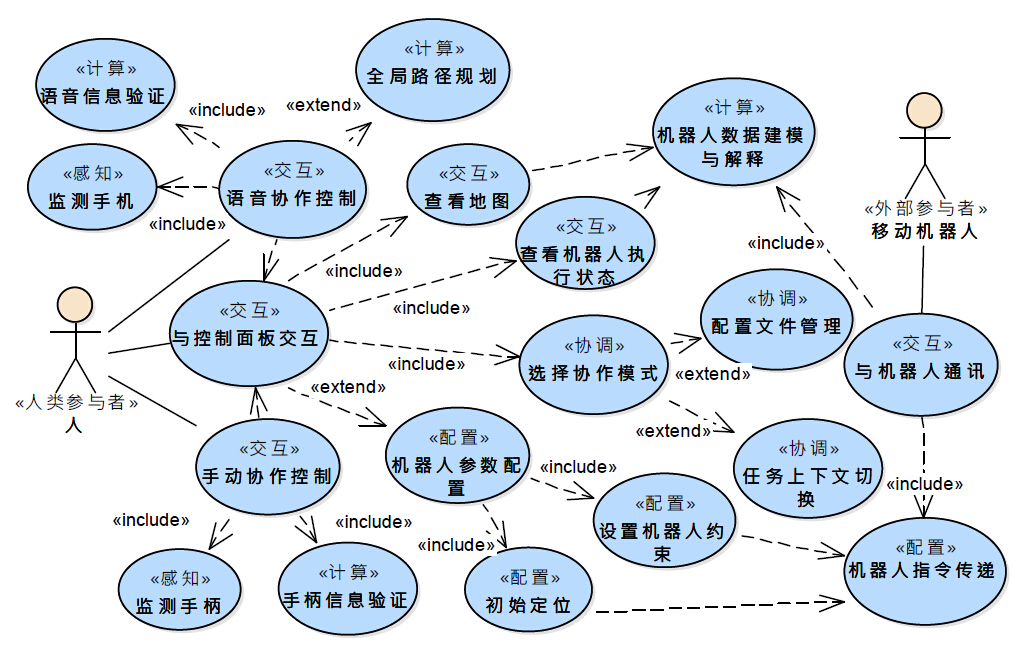
\includegraphics[scale=0.4]{./resource/graph/4.jpg}
\end{frame}
%--- Next Frame ---%
\begin{frame}[t]{组件图描述静态结构}
    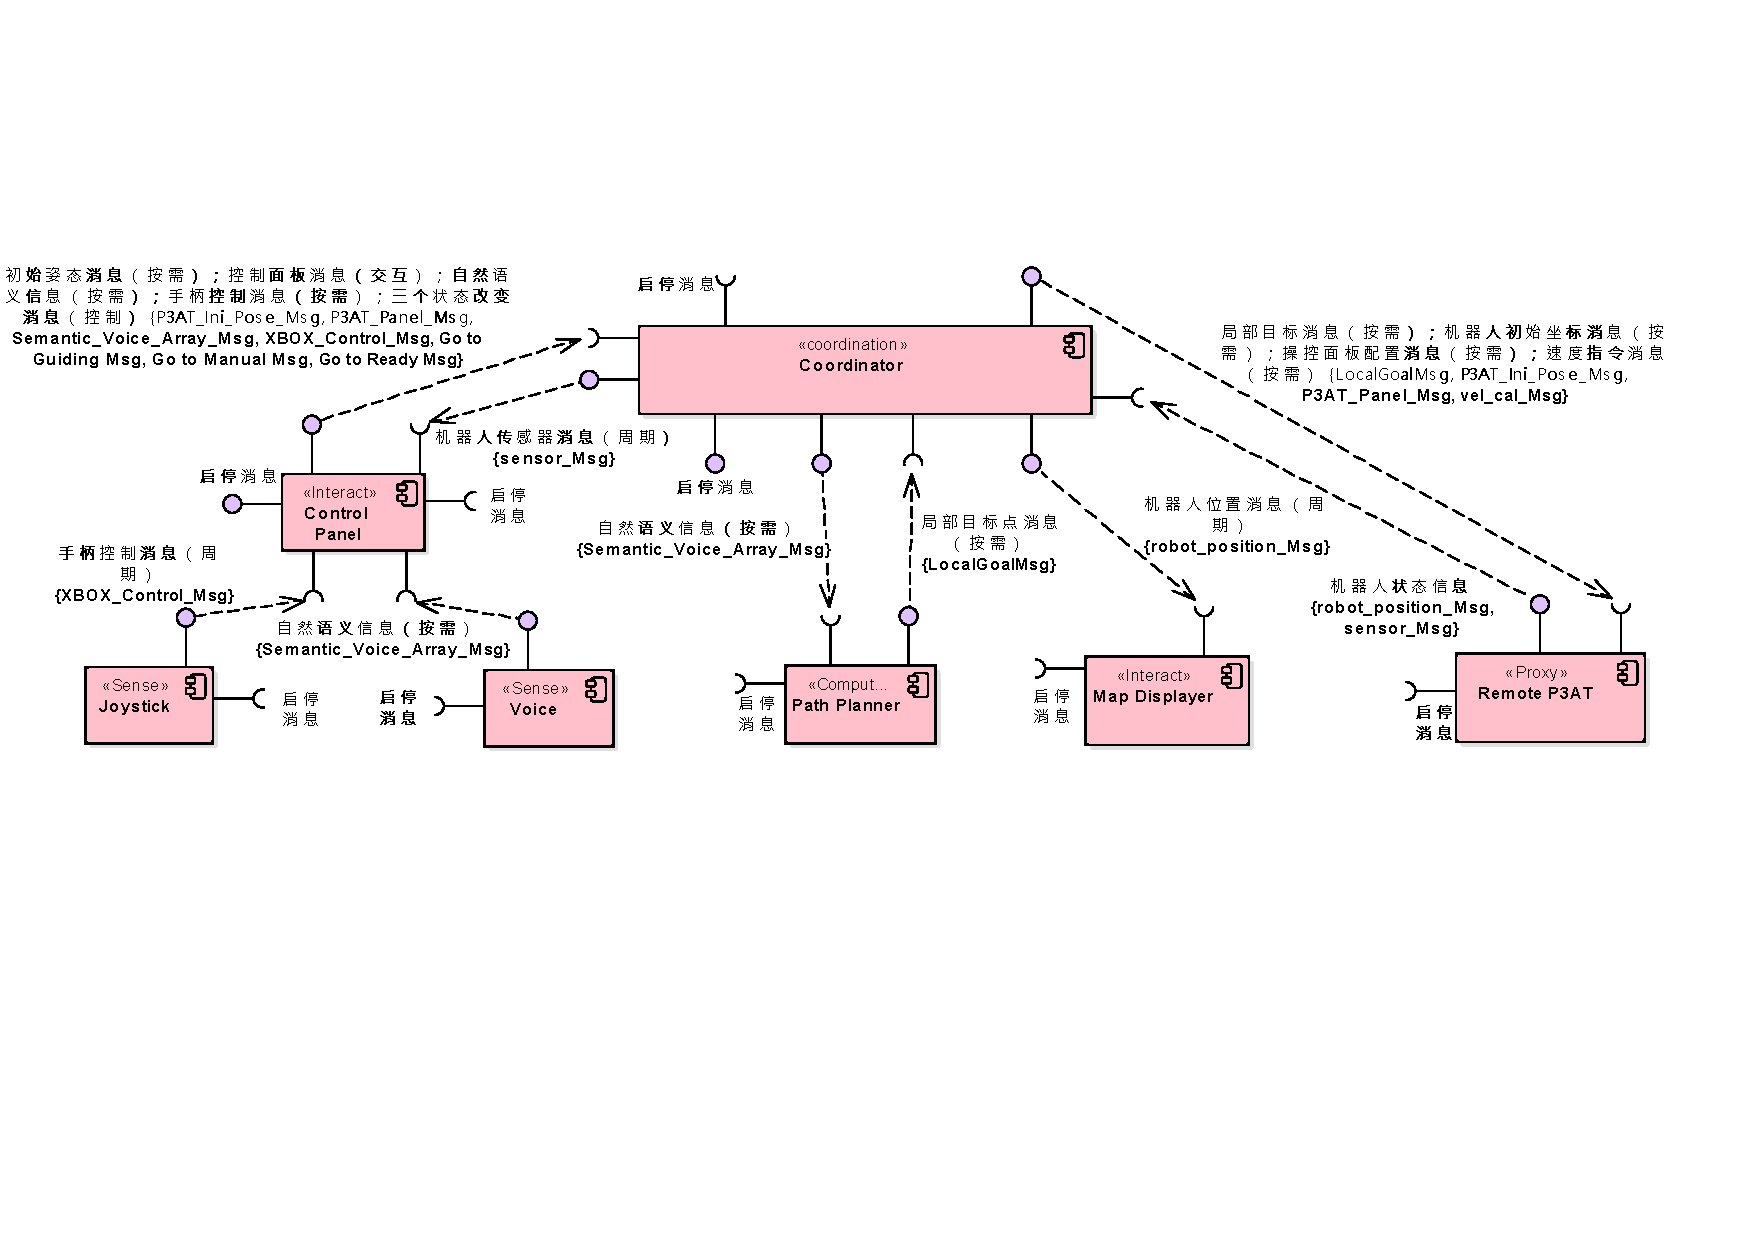
\includegraphics[scale=0.38]{./resource/graph/5.pdf}
\end{frame}
%--- Next Frame ---%
\begin{frame}[t]{顺序图描述动态结构}
    \href{./resource/files/sequence.pdf}{这是简化了的,点击打开详细图}
    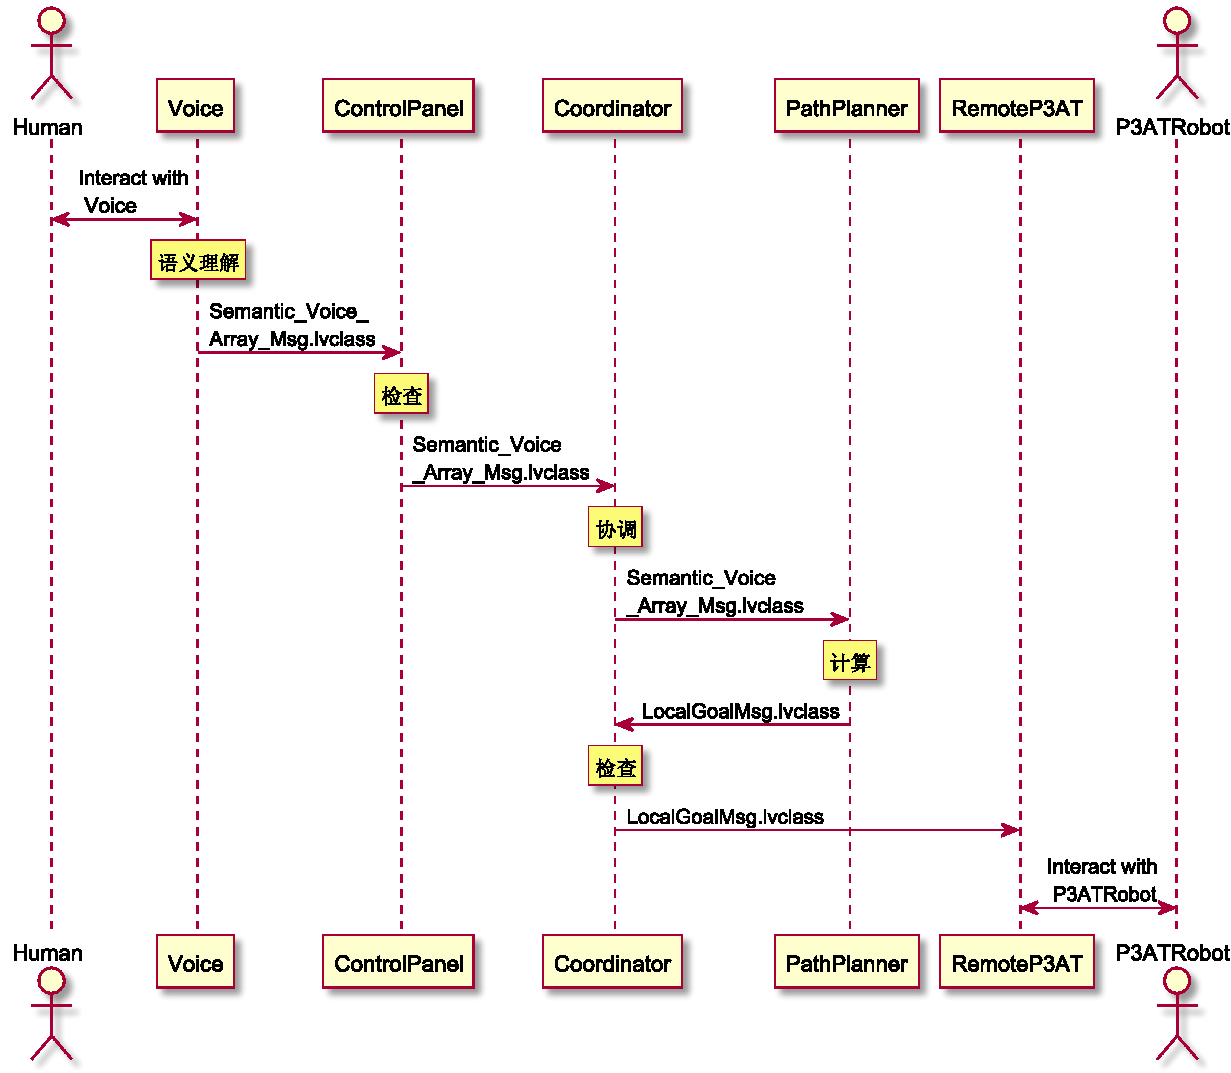
\includegraphics[scale=0.38]{./resource/graph/6.pdf}
\end{frame}
%--- Next Frame ---%
\begin{frame}[t]{类图描述内部结构}
    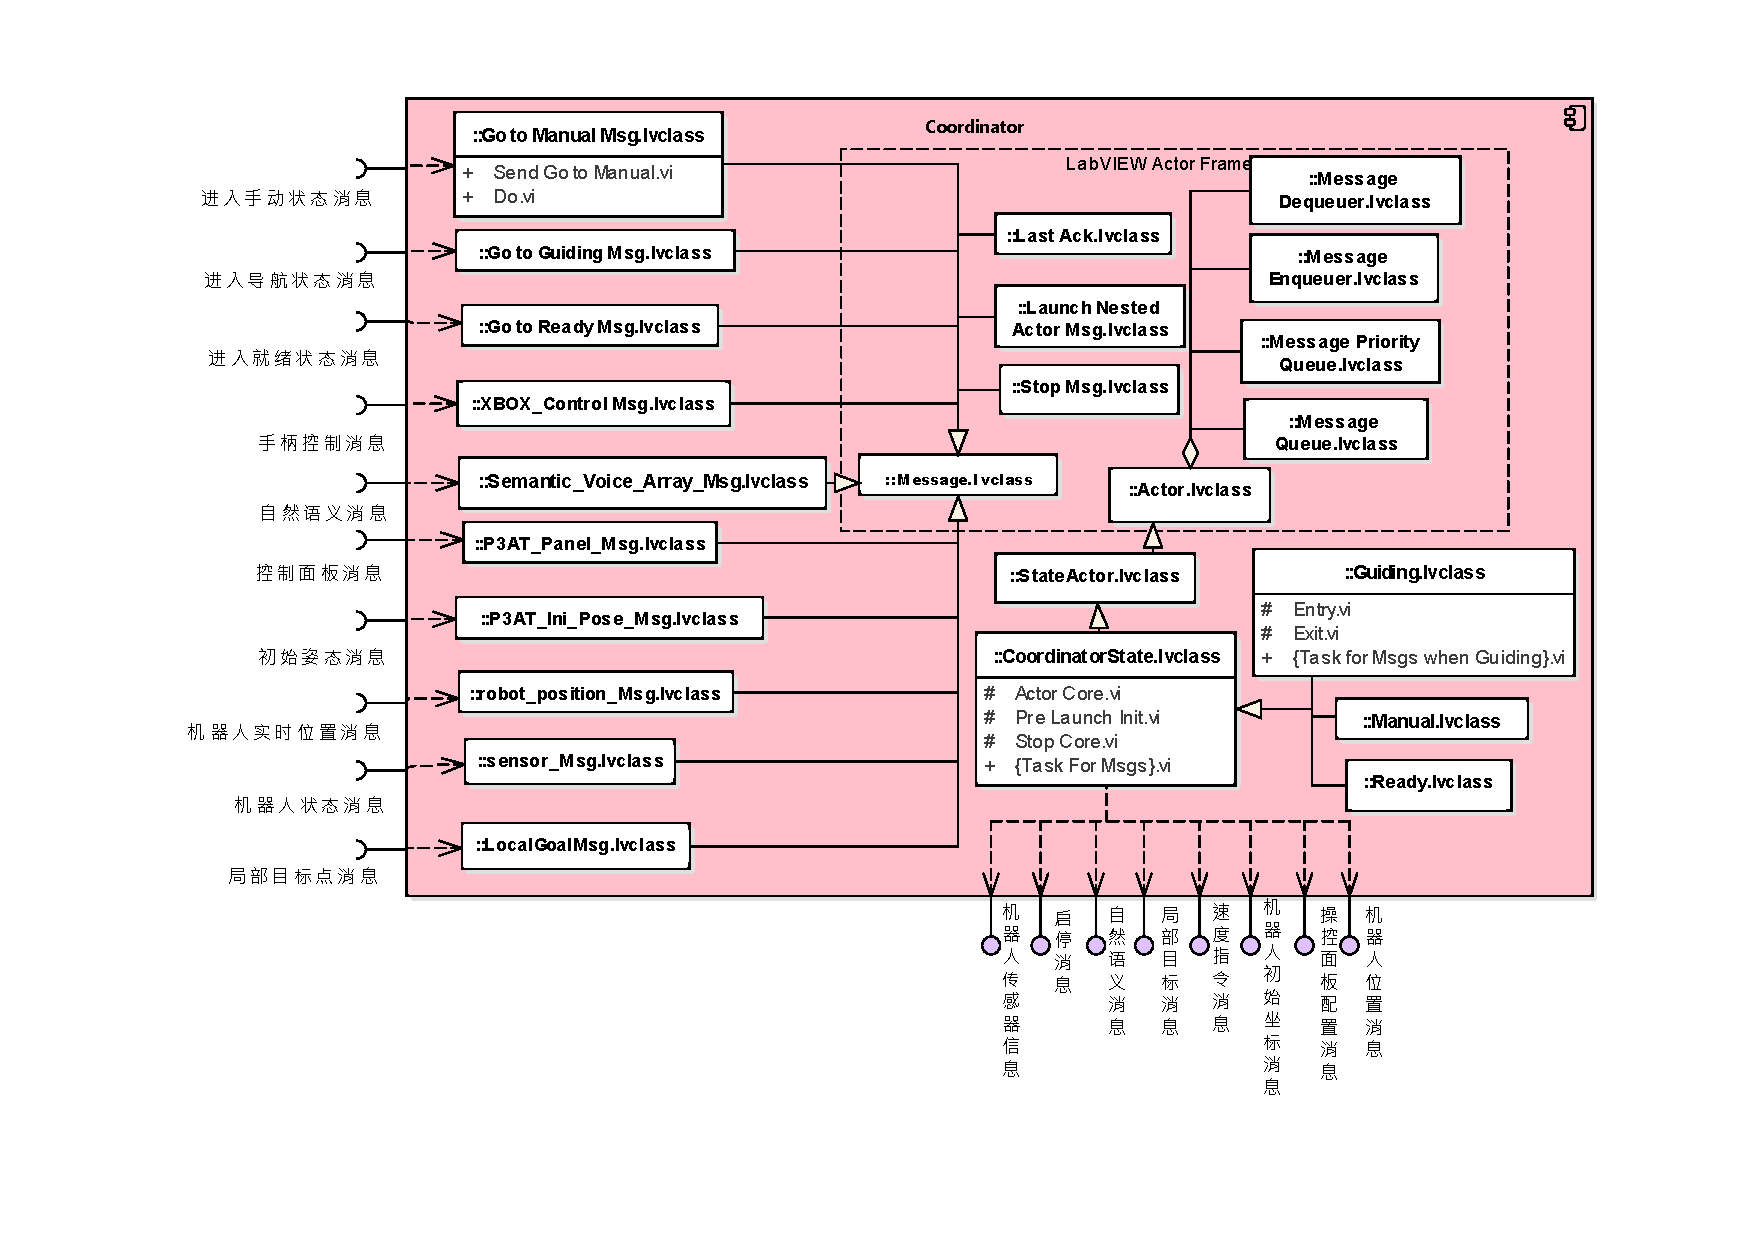
\includegraphics[scale=0.42]{./resource/graph/8.pdf}
\end{frame}
%--- Next Frame ---%
\begin{frame}[t]{2.3rosbridge client implementation in LabVIEW}
    \subsection{rosbridge client}
    \begin{itemize}
        \item 什么是rosbridge
            \begin{itemize}
                \item \href{http://wiki.ros.org/rosbridge_suite}{Rosbridge provides a JSON API to ROS functionality for non-ROS programs.
                There are a variety of front ends that interface with rosbridge, including a WebSocket server for web browsers to interact with.}
            \end{itemize}
        \item rosbridge通信规约
            \begin{itemize}
                \item \href{https://github.com/RobotWebTools/rosbridge_suite/blob/develop/ROSBRIDGE_PROTOCOL.md}{点击链接}
            \end{itemize}
        \item 使用LabVIEW tcp功能连接
        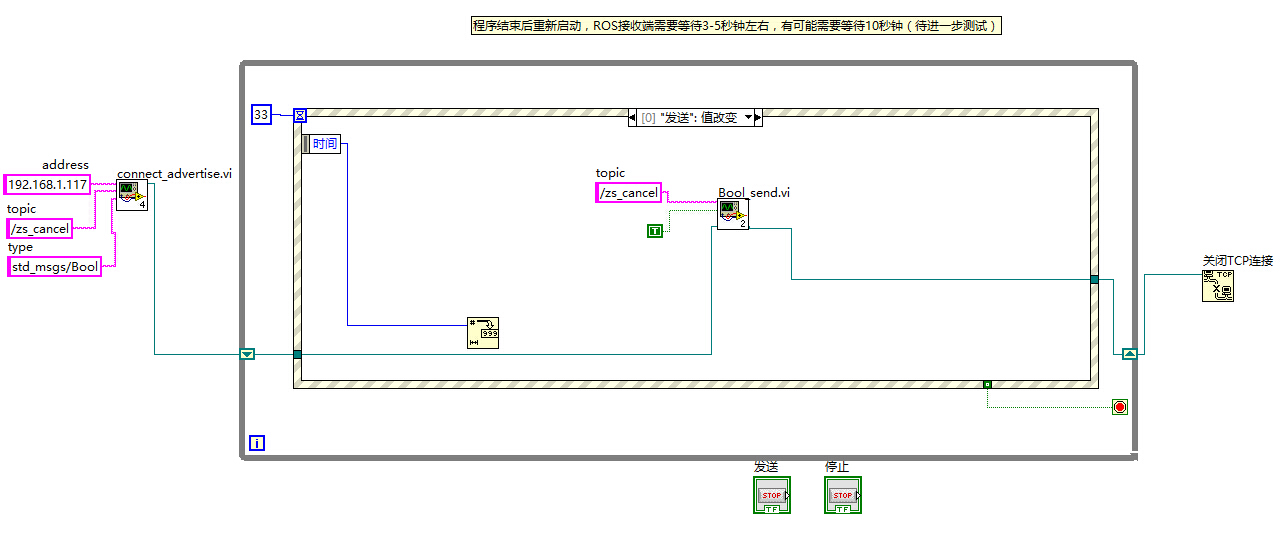
\includegraphics[scale=0.3]{./resource/graph/rosbridge.jpg}
    \end{itemize}
\end{frame}
% %--- Next Frame ---%
% \begin{frame}[t]{rosbridge client与ROS通信}
%     这里需要一张图片
% \end{frame}
%--- Next Frame ---%
\begin{frame}[t]{演示}
    \subsection{Video}
    \href{./resource/video/1.avi}{点击此处打开视频:}
    \begin{itemize}
        \item 1:40-3:30是配置和手动
        \item 之后是语音控制部分
    \end{itemize}
\end{frame}
%--- Next Frame ---%
\begin{frame}[t]{3.基于ROS的移动机器人实验系统设计和实现}
    \section{基于ROS的移动机器人实验系统设计与实现}
    \subsection{系统框架}
    ROS是一个开源的元级操作系统(后操作系统),
    提供类似于操作系统的服务,包括硬件抽象描述、底层驱动程序管理、共用功能的执行、程序间消息传递、程序发行包管理,
    它也提供一些工具和库用于获取、建立、编写和执行多机融合的程序。(摘自wikipedia)
    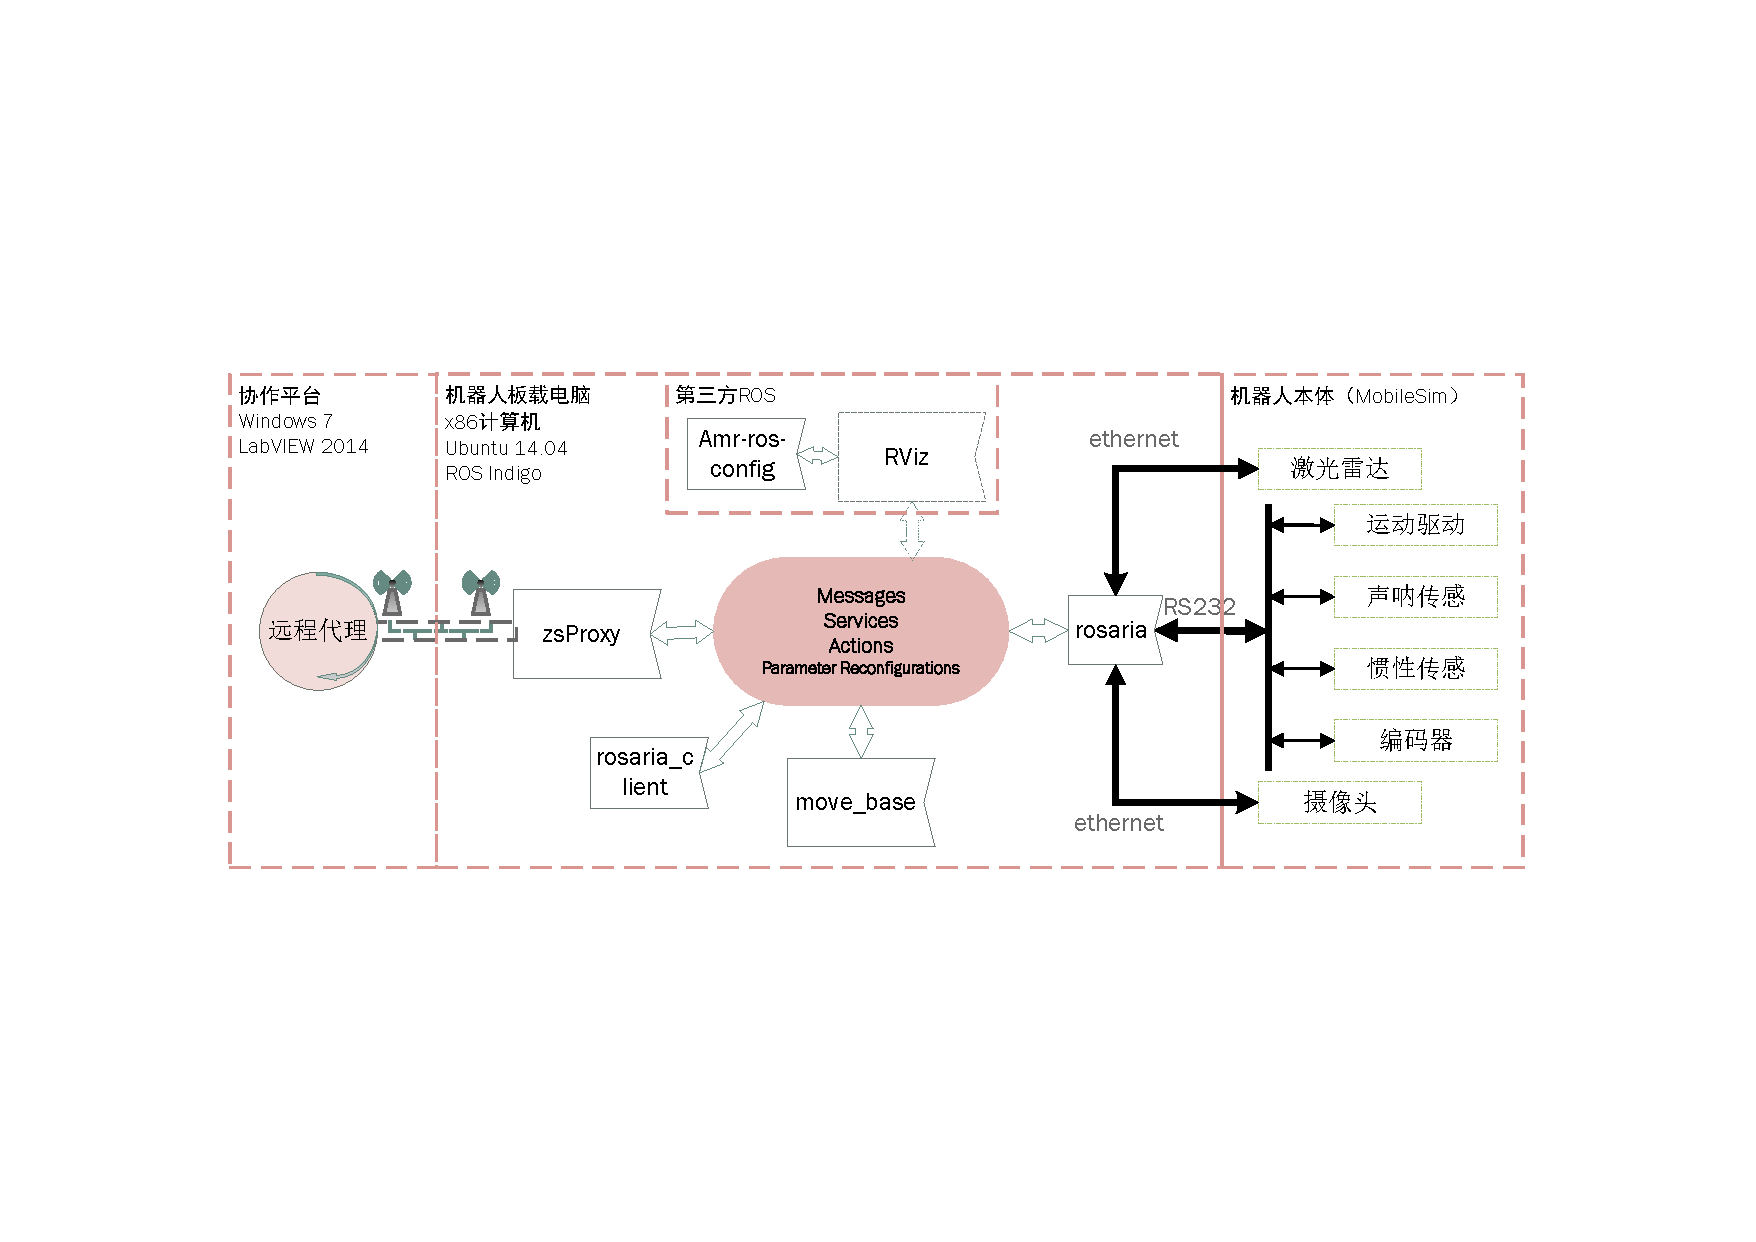
\includegraphics[scale=0.45]{./resource/graph/10-visio2010.pdf}
\end{frame}
%--- Next Frame ---%

\end{document}